% Created by tikzDevice version 0.12 on 2018-09-17 17:58:57
% !TEX encoding = UTF-8 Unicode
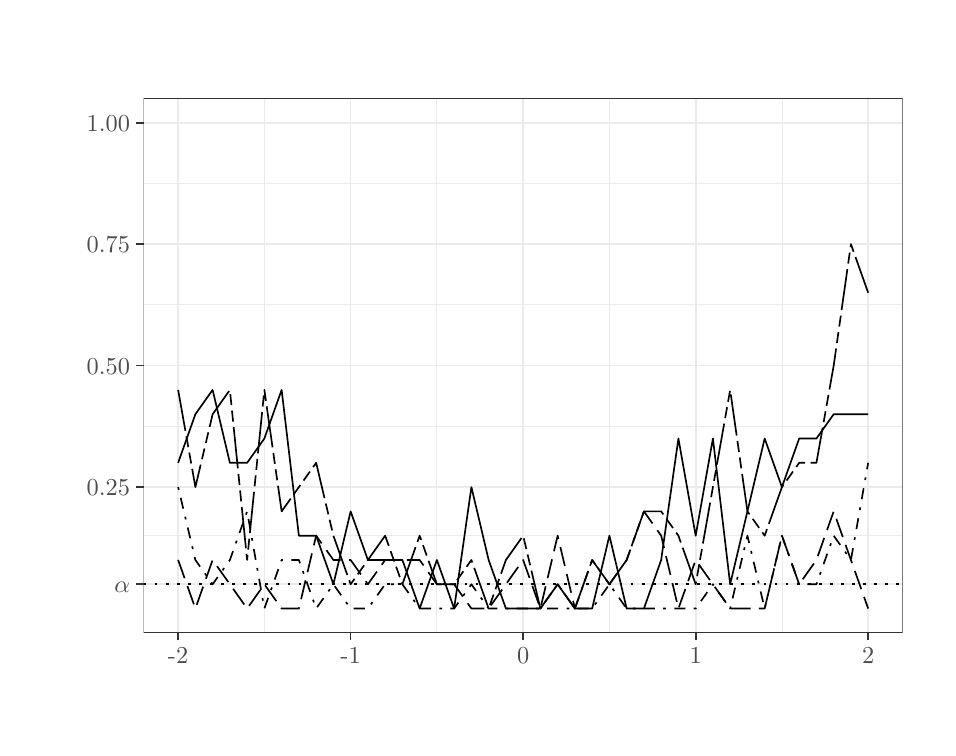
\begin{tikzpicture}[x=1pt,y=1pt]
\definecolor{fillColor}{RGB}{255,255,255}
\path[use as bounding box,fill=fillColor,fill opacity=0.00] (0,0) rectangle (325.21,252.94);
\begin{scope}
\path[clip] (  0.00,  0.00) rectangle (325.21,252.94);
\definecolor{drawColor}{RGB}{255,255,255}
\definecolor{fillColor}{RGB}{255,255,255}

\path[draw=drawColor,line width= 0.6pt,line join=round,line cap=round,fill=fillColor] (  0.00,  0.00) rectangle (325.21,252.94);
\end{scope}
\begin{scope}
\path[clip] ( 41.90, 34.26) rectangle (316.18,227.38);
\definecolor{fillColor}{RGB}{255,255,255}

\path[fill=fillColor] ( 41.90, 34.26) rectangle (316.18,227.38);
\definecolor{drawColor}{gray}{0.92}

\path[draw=drawColor,line width= 0.3pt,line join=round] ( 41.90, 69.37) --
	(316.18, 69.37);

\path[draw=drawColor,line width= 0.3pt,line join=round] ( 41.90,108.87) --
	(316.18,108.87);

\path[draw=drawColor,line width= 0.3pt,line join=round] ( 41.90,152.76) --
	(316.18,152.76);

\path[draw=drawColor,line width= 0.3pt,line join=round] ( 41.90,196.65) --
	(316.18,196.65);

\path[draw=drawColor,line width= 0.3pt,line join=round] ( 85.53, 34.26) --
	( 85.53,227.38);

\path[draw=drawColor,line width= 0.3pt,line join=round] (147.87, 34.26) --
	(147.87,227.38);

\path[draw=drawColor,line width= 0.3pt,line join=round] (210.21, 34.26) --
	(210.21,227.38);

\path[draw=drawColor,line width= 0.3pt,line join=round] (272.55, 34.26) --
	(272.55,227.38);

\path[draw=drawColor,line width= 0.6pt,line join=round] ( 41.90, 51.81) --
	(316.18, 51.81);

\path[draw=drawColor,line width= 0.6pt,line join=round] ( 41.90, 86.93) --
	(316.18, 86.93);

\path[draw=drawColor,line width= 0.6pt,line join=round] ( 41.90,130.82) --
	(316.18,130.82);

\path[draw=drawColor,line width= 0.6pt,line join=round] ( 41.90,174.71) --
	(316.18,174.71);

\path[draw=drawColor,line width= 0.6pt,line join=round] ( 41.90,218.60) --
	(316.18,218.60);

\path[draw=drawColor,line width= 0.6pt,line join=round] ( 54.37, 34.26) --
	( 54.37,227.38);

\path[draw=drawColor,line width= 0.6pt,line join=round] (116.70, 34.26) --
	(116.70,227.38);

\path[draw=drawColor,line width= 0.6pt,line join=round] (179.04, 34.26) --
	(179.04,227.38);

\path[draw=drawColor,line width= 0.6pt,line join=round] (241.38, 34.26) --
	(241.38,227.38);

\path[draw=drawColor,line width= 0.6pt,line join=round] (303.71, 34.26) --
	(303.71,227.38);
\definecolor{drawColor}{RGB}{0,0,0}

\path[draw=drawColor,line width= 0.6pt,dash pattern=on 1pt off 3pt on 4pt off 3pt ,line join=round] ( 54.37, 86.93) --
	( 60.60, 60.59) --
	( 66.83, 51.81) --
	( 73.07, 60.59) --
	( 79.30, 78.15) --
	( 85.53, 43.04) --
	( 91.77, 60.59) --
	( 98.00, 60.59) --
	(104.24, 43.04) --
	(110.47, 51.81) --
	(116.70, 43.04) --
	(122.94, 43.04) --
	(129.17, 51.81) --
	(135.40, 51.81) --
	(141.64, 43.04) --
	(147.87, 43.04) --
	(154.10, 43.04) --
	(160.34, 51.81) --
	(166.57, 43.04) --
	(172.81, 43.04) --
	(179.04, 43.04) --
	(185.27, 43.04) --
	(191.51, 43.04) --
	(197.74, 43.04) --
	(203.97, 43.04) --
	(210.21, 51.81) --
	(216.44, 43.04) --
	(222.68, 43.04) --
	(228.91, 43.04) --
	(235.14, 43.04) --
	(241.38, 43.04) --
	(247.61, 51.81) --
	(253.84, 43.04) --
	(260.08, 69.37) --
	(266.31, 43.04) --
	(272.55, 69.37) --
	(278.78, 51.81) --
	(285.01, 51.81) --
	(291.25, 69.37) --
	(297.48, 60.59) --
	(303.71, 95.70);

\path[draw=drawColor,line width= 0.6pt,dash pattern=on 15pt off 2pt on 4pt off 2pt on 4pt off 2pt ,line join=round] ( 54.37,122.04) --
	( 60.60, 86.93) --
	( 66.83,113.26) --
	( 73.07,122.04) --
	( 79.30, 60.59) --
	( 85.53,122.04) --
	( 91.77, 78.15) --
	( 98.00, 86.93) --
	(104.24, 95.70) --
	(110.47, 69.37) --
	(116.70, 51.81) --
	(122.94, 60.59) --
	(129.17, 69.37) --
	(135.40, 51.81) --
	(141.64, 69.37) --
	(147.87, 51.81) --
	(154.10, 51.81) --
	(160.34, 60.59) --
	(166.57, 43.04) --
	(172.81, 60.59) --
	(179.04, 69.37) --
	(185.27, 43.04) --
	(191.51, 51.81) --
	(197.74, 43.04) --
	(203.97, 60.59) --
	(210.21, 51.81) --
	(216.44, 60.59) --
	(222.68, 78.15) --
	(228.91, 78.15) --
	(235.14, 69.37) --
	(241.38, 51.81) --
	(247.61, 86.93) --
	(253.84,122.04) --
	(260.08, 78.15) --
	(266.31, 69.37) --
	(272.55, 86.93) --
	(278.78, 95.70) --
	(285.01, 95.70) --
	(291.25,130.82) --
	(297.48,174.71) --
	(303.71,157.15);

\path[draw=drawColor,line width= 0.6pt,dash pattern=on 7pt off 3pt ,line join=round] ( 54.37, 60.59) --
	( 60.60, 43.04) --
	( 66.83, 60.59) --
	( 73.07, 51.81) --
	( 79.30, 43.04) --
	( 85.53, 51.81) --
	( 91.77, 43.04) --
	( 98.00, 43.04) --
	(104.24, 69.37) --
	(110.47, 60.59) --
	(116.70, 60.59) --
	(122.94, 51.81) --
	(129.17, 60.59) --
	(135.40, 60.59) --
	(141.64, 60.59) --
	(147.87, 51.81) --
	(154.10, 51.81) --
	(160.34, 43.04) --
	(166.57, 43.04) --
	(172.81, 51.81) --
	(179.04, 60.59) --
	(185.27, 43.04) --
	(191.51, 69.37) --
	(197.74, 43.04) --
	(203.97, 60.59) --
	(210.21, 51.81) --
	(216.44, 60.59) --
	(222.68, 78.15) --
	(228.91, 69.37) --
	(235.14, 43.04) --
	(241.38, 60.59) --
	(247.61, 51.81) --
	(253.84, 43.04) --
	(260.08, 43.04) --
	(266.31, 43.04) --
	(272.55, 69.37) --
	(278.78, 51.81) --
	(285.01, 60.59) --
	(291.25, 78.15) --
	(297.48, 60.59) --
	(303.71, 43.04);

\path[draw=drawColor,line width= 0.6pt,line join=round] ( 54.37, 95.70) --
	( 60.60,113.26) --
	( 66.83,122.04) --
	( 73.07, 95.70) --
	( 79.30, 95.70) --
	( 85.53,104.48) --
	( 91.77,122.04) --
	( 98.00, 69.37) --
	(104.24, 69.37) --
	(110.47, 51.81) --
	(116.70, 78.15) --
	(122.94, 60.59) --
	(129.17, 60.59) --
	(135.40, 60.59) --
	(141.64, 43.04) --
	(147.87, 60.59) --
	(154.10, 43.04) --
	(160.34, 86.93) --
	(166.57, 60.59) --
	(172.81, 43.04) --
	(179.04, 43.04) --
	(185.27, 43.04) --
	(191.51, 51.81) --
	(197.74, 43.04) --
	(203.97, 43.04) --
	(210.21, 69.37) --
	(216.44, 43.04) --
	(222.68, 43.04) --
	(228.91, 60.59) --
	(235.14,104.48) --
	(241.38, 69.37) --
	(247.61,104.48) --
	(253.84, 51.81) --
	(260.08, 78.15) --
	(266.31,104.48) --
	(272.55, 86.93) --
	(278.78,104.48) --
	(285.01,104.48) --
	(291.25,113.26) --
	(297.48,113.26) --
	(303.71,113.26);

\path[draw=drawColor,line width= 0.6pt,dash pattern=on 1pt off 3pt ,line join=round] ( 41.90, 51.81) -- (316.18, 51.81);
\definecolor{drawColor}{gray}{0.20}

\path[draw=drawColor,line width= 0.6pt,line join=round,line cap=round] ( 41.90, 34.26) rectangle (316.18,227.38);
\end{scope}
\begin{scope}
\path[clip] (  0.00,  0.00) rectangle (325.21,252.94);
\definecolor{drawColor}{gray}{0.30}

\node[text=drawColor,anchor=base east,inner sep=0pt, outer sep=0pt, scale=  0.88] at ( 36.95, 48.78) {$\alpha$};

\node[text=drawColor,anchor=base east,inner sep=0pt, outer sep=0pt, scale=  0.88] at ( 36.95, 83.90) {$0.25$};

\node[text=drawColor,anchor=base east,inner sep=0pt, outer sep=0pt, scale=  0.88] at ( 36.95,127.79) {$0.50$};

\node[text=drawColor,anchor=base east,inner sep=0pt, outer sep=0pt, scale=  0.88] at ( 36.95,171.68) {$0.75$};

\node[text=drawColor,anchor=base east,inner sep=0pt, outer sep=0pt, scale=  0.88] at ( 36.95,215.57) {$1.00$};
\end{scope}
\begin{scope}
\path[clip] (  0.00,  0.00) rectangle (325.21,252.94);
\definecolor{drawColor}{gray}{0.20}

\path[draw=drawColor,line width= 0.6pt,line join=round] ( 39.15, 51.81) --
	( 41.90, 51.81);

\path[draw=drawColor,line width= 0.6pt,line join=round] ( 39.15, 86.93) --
	( 41.90, 86.93);

\path[draw=drawColor,line width= 0.6pt,line join=round] ( 39.15,130.82) --
	( 41.90,130.82);

\path[draw=drawColor,line width= 0.6pt,line join=round] ( 39.15,174.71) --
	( 41.90,174.71);

\path[draw=drawColor,line width= 0.6pt,line join=round] ( 39.15,218.60) --
	( 41.90,218.60);
\end{scope}
\begin{scope}
\path[clip] (  0.00,  0.00) rectangle (325.21,252.94);
\definecolor{drawColor}{gray}{0.20}

\path[draw=drawColor,line width= 0.6pt,line join=round] ( 54.37, 31.51) --
	( 54.37, 34.26);

\path[draw=drawColor,line width= 0.6pt,line join=round] (116.70, 31.51) --
	(116.70, 34.26);

\path[draw=drawColor,line width= 0.6pt,line join=round] (179.04, 31.51) --
	(179.04, 34.26);

\path[draw=drawColor,line width= 0.6pt,line join=round] (241.38, 31.51) --
	(241.38, 34.26);

\path[draw=drawColor,line width= 0.6pt,line join=round] (303.71, 31.51) --
	(303.71, 34.26);
\end{scope}
\begin{scope}
\path[clip] (  0.00,  0.00) rectangle (325.21,252.94);
\definecolor{drawColor}{gray}{0.30}

\node[text=drawColor,anchor=base,inner sep=0pt, outer sep=0pt, scale=  0.88] at ( 54.37, 23.25) {-2};

\node[text=drawColor,anchor=base,inner sep=0pt, outer sep=0pt, scale=  0.88] at (116.70, 23.25) {-1};

\node[text=drawColor,anchor=base,inner sep=0pt, outer sep=0pt, scale=  0.88] at (179.04, 23.25) {0};

\node[text=drawColor,anchor=base,inner sep=0pt, outer sep=0pt, scale=  0.88] at (241.38, 23.25) {1};

\node[text=drawColor,anchor=base,inner sep=0pt, outer sep=0pt, scale=  0.88] at (303.71, 23.25) {2};
\end{scope}
\end{tikzpicture}
